\documentclass{modernsimplecv}
% try out different fonts: classic, fira, raleway, chivo
\usepackage[utf8]{inputenc}
\usepackage[OT1]{fontenc}
\usepackage[
    reset,
    a4paper,
    margin=0.5cm, 
    top=0.1cm,
    nomarginpar,% We don't want any margin paragraphs
    textwidth=10cm,% Set \textwidth to 10cm
    headheight=10mm,
    includefoot
]{geometry}

% ------------------------------------------------------------------------------------
% you can try out different fonts here by commenting the following lines in and out
% -----------------------------------------------------------------------------------
\usepackage[default]{raleway}
% \usepackage[sfdefault]{FiraSans} %% option 'sfdefault' activates Fira Sans as the default text font\renewcommand*\oldstylenums[1]{{\firaoldstyle #1}}\normalfont
% \usepackage[familydefault,light]{Chivo} 
% \usepackage[sfdefault,light,condensed]{roboto}
% \usepackage[default]{cantarell}
% \usepackage[sfdefault]{AlegreyaSans}


\usepackage{beuron}
\usepackage{LobsterTwo}%if not suposed to be main font, load other main font after this

\usepackage{worldflags}

%------------------------------------------------------------------ Variables

\newlength{\rightcolwidth}
\newlength{\leftcolwidth}
\setlength{\leftcolwidth}{0.45\textwidth}
\setlength{\rightcolwidth}{0.495\textwidth}

%------------------------------------------------------------------
\title{Razvan-Puha-CV}
\author{\LaTeX{} Razvan Puha}
\date{December 2023}

\pagestyle{empty}
\begin{document}
    \pagestyle{fancy}
    \fancyhf{} % clear existing header/footer entries
    \fancyfoot[C]{
        \fontfamily{\sfdefault}
        \selectfont \color{black!70}
        \small Razvan Puha 
        \icon{\faBriefcase}{black}{\small Administrator@PHR Soft Solutions} 
        \icon{\faPhone}{black}{\href{tel:+40770839944}{+40 770 839 944}} 
        \icon{\faAt}{black}{
            \href{mailto:puha.razvan@phrsoftsolutions.com}{puha.razvan@phrsoftsolutions.com}
        } 
    }
    \begin{minipage}[t]{\textwidth}
        \vspace{0pt} % Trick for alignment
        \begin{shaded*}
            \begin{multicols}{2}
                \begin{minipage}[t]{0.4\textwidth}
                    \vspace{0pt} % Trick for alignment
                    % here the fancy font can be taken out by removing \LobsterTwo
                    {
                        \par\centering\huge\LobsterTwo{Razvan Puha}
                    } \\[0.3cm]
                    
                    \faGlobe~ Nationality: \worldflag[width=3mm]{RO} \\
                    \faLocationArrow~ Bucharest, Romania \\
            
                    {
                        \small
                        \faComments~ \underline{Languages:} 
                        \begin{itemize}
                            \item \emph{Romanian} - native
                            \item \emph{English} - B2
                        \end{itemize}
                    }
                \end{minipage}
            
                \hfill
            
                \begin{minipage}[t]{0.4\textwidth}
                    \vspace{0pt} % Trick for alignment
                    \vspace{1cm}
                    \faPhone~ \href{tel:+40770839944}{+40 770 839 944} \\
                    \faAt~ \href{mailto:puha.razvan@phrsoftsolutions.com}{puha.razvan@phrsoftsolutions.com} \\
                    
                    \faGithub~ \href{https://github.com/razvan-puha}{@razvan-puha} \\
                    \faLinkedin~ \href{https://www.linkedin.com/in/razvan-petru-puha}{@razvan-puha} \\
                    \faCalendar~ \href{https://calendly.com/puha-razvan-office}{calendly.com/razvan-puha}

                \end{minipage}
                
                \hfill
    
                % Might add the profile picture later
                % \begin{minipage}[t]{0.1\textwidth}
                %     \vspace{0pt} % Trick for alignment
                %     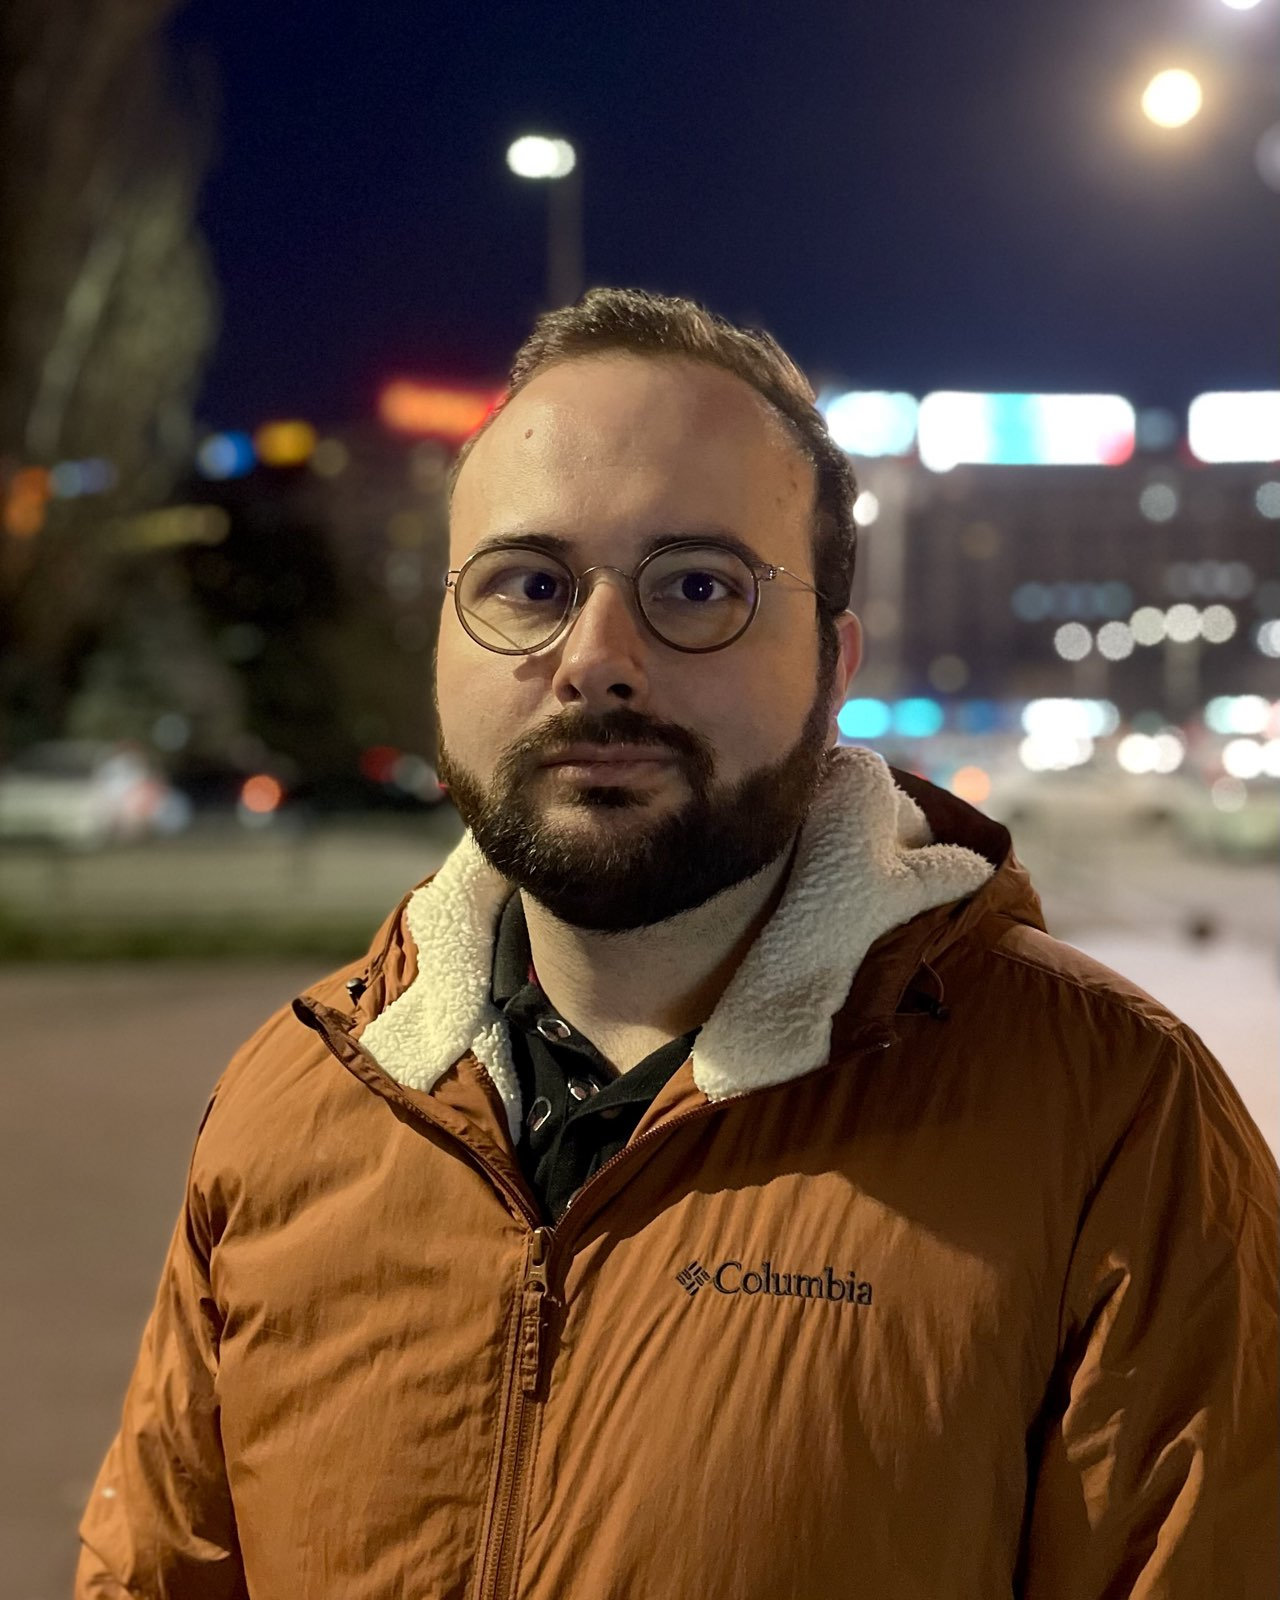
\includegraphics[width=\textwidth]{Razvan.jpg}
                % \end{minipage}
        \end{multicols}
        \end{shaded*}
    \end{minipage}\\[3pt]
    
    
    %------------------------------------------------
    
    \subsection*{}
    \vspace{-3em}
    
    \setlength{\columnsep}{2cm}
    \columnratio{0.45}[0.47]
    \begin{paracol}{2}
    \hbadness5000
    %\backgroundcolor{c[1]}[rgb]{1,1,0.8} % cream yellow for column-1 %\backgroundcolor{g}[rgb]{0.8,1,1} % \backgroundcolor{l}[rgb]{0,0,0.7} % dark blue for left margin
    
    \paracolbackgroundoptions
    
    % 0.9,0.9,0.9 -- 0.8,0.8,0.8
    
    
    \footnotesize
    {
        \begin{minipage}[t]{\leftcolwidth}
            \small
            \section*{\faNewspaperO~ Work Experience - Contractor}
            \begin{tabular}{p{3em} | p{0.6\textwidth} c}
                \cvevent{2023}{Wisesystems}{Backend}{Remote}{
                    \color{black!70}\footnotesize During my period here, I helped in splitting the old APIs (built as a distributed monolith) into self-contained, independently deployable microservices, in order to maintain consistency with the new APIs being added.\newline
                    
                    I was also in charge of adding new features to the existing APIs, along with providing support to the frontend/game designers team; with the requirements consistently changing, I’ve managed to keep the same level of availability and consistency of the backend services.
                }{
\includegraphics[scale=0.15]{logo.png}} \\
                \cvevent{2022--2023}{Neckdei Solutions}{Full-Stack}{Remote}{
                    \color{black!70}\footnotesize Was responsible for the entire project from scratch, working as sole developer.\newline
                    
                    Built a platform for improving relations between institutions (public and private) and possible clients; the users can contact, leave feedback/suggestions, etc. to the institutions and track updates on those operations.\newline
                }{
\includegraphics[scale=0.15]{logo.png}} \\
                \cvevent{2021--2022}{Adobe}{Full-Stack}{Remote}{
                    \color{black!70}\footnotesize Helped in rewriting the social sign-in/sign-up functionality for Google IDP.\newline
                    
                    Offered support \& optimized/developed new frontend/backend functionalities for the Identity services (services used for the authorization \& authentication of the clients across the Adobe platform)
                }{
\includegraphics[scale=0.15]{logo.png}} \\
                \cvevent{2021}{Metro Systems}{Backend}{Remote}{
                    \color{black!70}\footnotesize Worked with a collection of microservices that provided the clients the
                    possibility to store documents \& receive notifications whenever the documents that they are following were updated.\newline
                    
                    Managed to keep the same performances, disregarding the traffic/volume of data present inside the product (at the moment of my joining it was already about a few TB of data and 20k-30k+ requests daily)
                }{
\includegraphics[scale=0.15]{logo.png}} \\
            \end{tabular}
        \end{minipage}
    
        \bigskip
    
        \begin{minipage}[t]{\leftcolwidth}
            \vspace{0.2cm} % For alignment
            \small
            \section*{\faNewspaperO~ Work Experience - Employee}
            \begin{tabular}{p{3em} | p{0.6\textwidth} c}
                \cvevent{2019--2020}{Cognizant Softvision}{Backend}{Bucharest/Remote}{
                    \color{black!70}\footnotesize Developed a REST API that provides useful information related to the investment in cocoa industry. \newline
                    Java 8, Spring, Hibernate, PostgreSQL, Drone, Microsoft Azure, Junit, Mockito
                }{
\includegraphics[scale=0.03]{Cognizant.png}} \\
                \cvevent{2018--2019}{Luxoft}{Backend}{Bucharest, RO}{
                    \color{black!70}\footnotesize Developed \& offered support for a test library for the client's main financial product.\newline
                    Java SE 8, Maven, Perforce, Lombok, Jenkins, Jira, JAXB, Jackson, JUnit, Mockito
                }{
\includegraphics[scale=0.5]{luxoft.png}}\\
                \cvevent{2015--2018}{Unicredit}{Backend}{Iasi, RO}{
                    \color{black!70}\footnotesize Java SE 7, Maven, Subversion, Oracle DB, JasperReports
                }{
\includegraphics[scale=0.5]{unicredit.png}}
            \end{tabular}
            
            % \bigskip
        \end{minipage}
    
    }
        %-----------------------------------------------------------
        \switchcolumn
    
        \begin{minipage}[t]{\rightcolwidth}
            \small
            \section*{\hspace{1mm}\faLaptop~ Personal Projects} 
            
            \begin{tabular}{p{3em} | p{0.6\textwidth} c}
                \personalproject{2023}{Archive Utilitary}{
                    \color{black!70}\footnotesize A utility tool for a small family business which does archive document organization, helping them to transition from traditional Excel-style databases to a more modern, contemporary look.\newline\newline
                    \color{black!70}\footnotesize Offering a better UI/UX than Excel spreadsheets, this tool also comes along with a couple of additional operations that can be done for every archive: generate labels, inventories, selection report etc.
                }{logo.png} \\
            \end{tabular}
        
        \end{minipage}
    
        \bigskip
    
        \begin{minipage}[t]{\rightcolwidth}
            \small
            \section*{\hspace{2mm}\faInfo~ About me}
            
            Backend Engineer with over 8 years of experience in developing desktop/web/mobile applications, with a keen and active interest in full-stack development in the last 2 years, currently activating as a contractor/freelancer.
        \end{minipage}
    
        \bigskip
    
        \begin{minipage}[t]{\rightcolwidth}
            \small
            \section{\hspace{1mm}\faCogs~ Programming} 
            {
                \small
                I've worked with various product teams, with sizes reaching from a sole developer to having more than 10-15 colleagues.\\
                
                I have experience in developing desktop, web and mobile applications; I've previously worked with monoliths, as well as with APIs and microservices. \\
                
                I'm able to provide my expertise in backend/frontend or even DevOps if it's required. \\
                
                I'm able to work in the following environments/use the following languages and tools at the moment:
            }
        \end{minipage}\\
    
        \hspace{2em}
    
        \begin{skillsection}{\rightcolwidth}
            \cvitem{\faStar\faStar\faStar\faStar\faStarO}{Spring}
            \cvitem{\faStar\faStar\faStar\faStar\faStarHalfO}{Java} \\
            \cvitem{\faStar\faStar\faStar\faStar\faStarO}{Hibernate}
            \cvitem{\faStar\faStar\faStar\faStar\faStarO}{SQL} \\
            \cvitem{\faStar\faStar\faStar\faStar\faStarO}{PostgreSQL}
            \cvitem{\faStar\faStar\faStar\faStarO\faStarO}{Javascript/Typescript} \\
            \cvitem{\faStar\faStar\faStar\faStar\faStarO}{Git}
            \cvitem{\faStar\faStar\faStar\faStarO\faStarO}{Golang} \\
            \cvitem{\faStar\faStar\faStar\faStarHalfO\faStarO}{React} \\
            \cvitem{\faStar\faStar\faStar\faStarO\faStarO}{React Native}
            \cvitem{\faStar\faStar\faStar\faStarO\faStarO}{GCP} \\
            \cvitem{\faStar\faStar\faStar\faStarO\faStarO}{Docker}
            \cvitem{\faStar\faStar\faStarHalfO\faStarO\faStarO}{AWS} \\
            \cvitem{\faStar\faStar\faStarO\faStarO\faStarO}{Kubernetes} \\
            \cvitem{\faStar\faStar\faStarO\faStarO\faStarO}{Apache Kafka} \\
            \cvitem{\faStar\faStar\faStarO\faStarO\faStarO}{Next.js} \\
        \end{skillsection}
    
        \vspace{2em}
        \bigskip
    
    \end{paracol}
\end{document}
